\section{Evalution}
\label{evaluation} 
In this section, we evaluate the algorithms proposed on a controlled testbed.

Our experimental tests were performed using two lenovo T430 laptops running debian (A and B), a BISmark access gateway \cite{sundaresan2011broadband} that has an OpenWRT-based platform for performing measurements (R), an OpenWRT-router used as a control router to limit access uplink and downlink bandwidth (Q), and a server machine with access to the Internet, running debian (S). Our experiments confirmed that TCP throughput over each link can be accurately measured to 90\% of the capacity using 4 parallel threads with a duration of 5 seconds.

We use a custom tc script with netem \cite{netem} on the control router to change access link bandwidth settings, and distance the wireless clients (A and B) to control the wireless channel. Our results indicate that the bandwidth based algorithms presented in \ref{bandwidth} can find the bottleneck accurately within 3 Mbps (Fig. \ref{fig:throughput_vs_bottleneck}).

\begin{figure}[!ht]
  \centering
  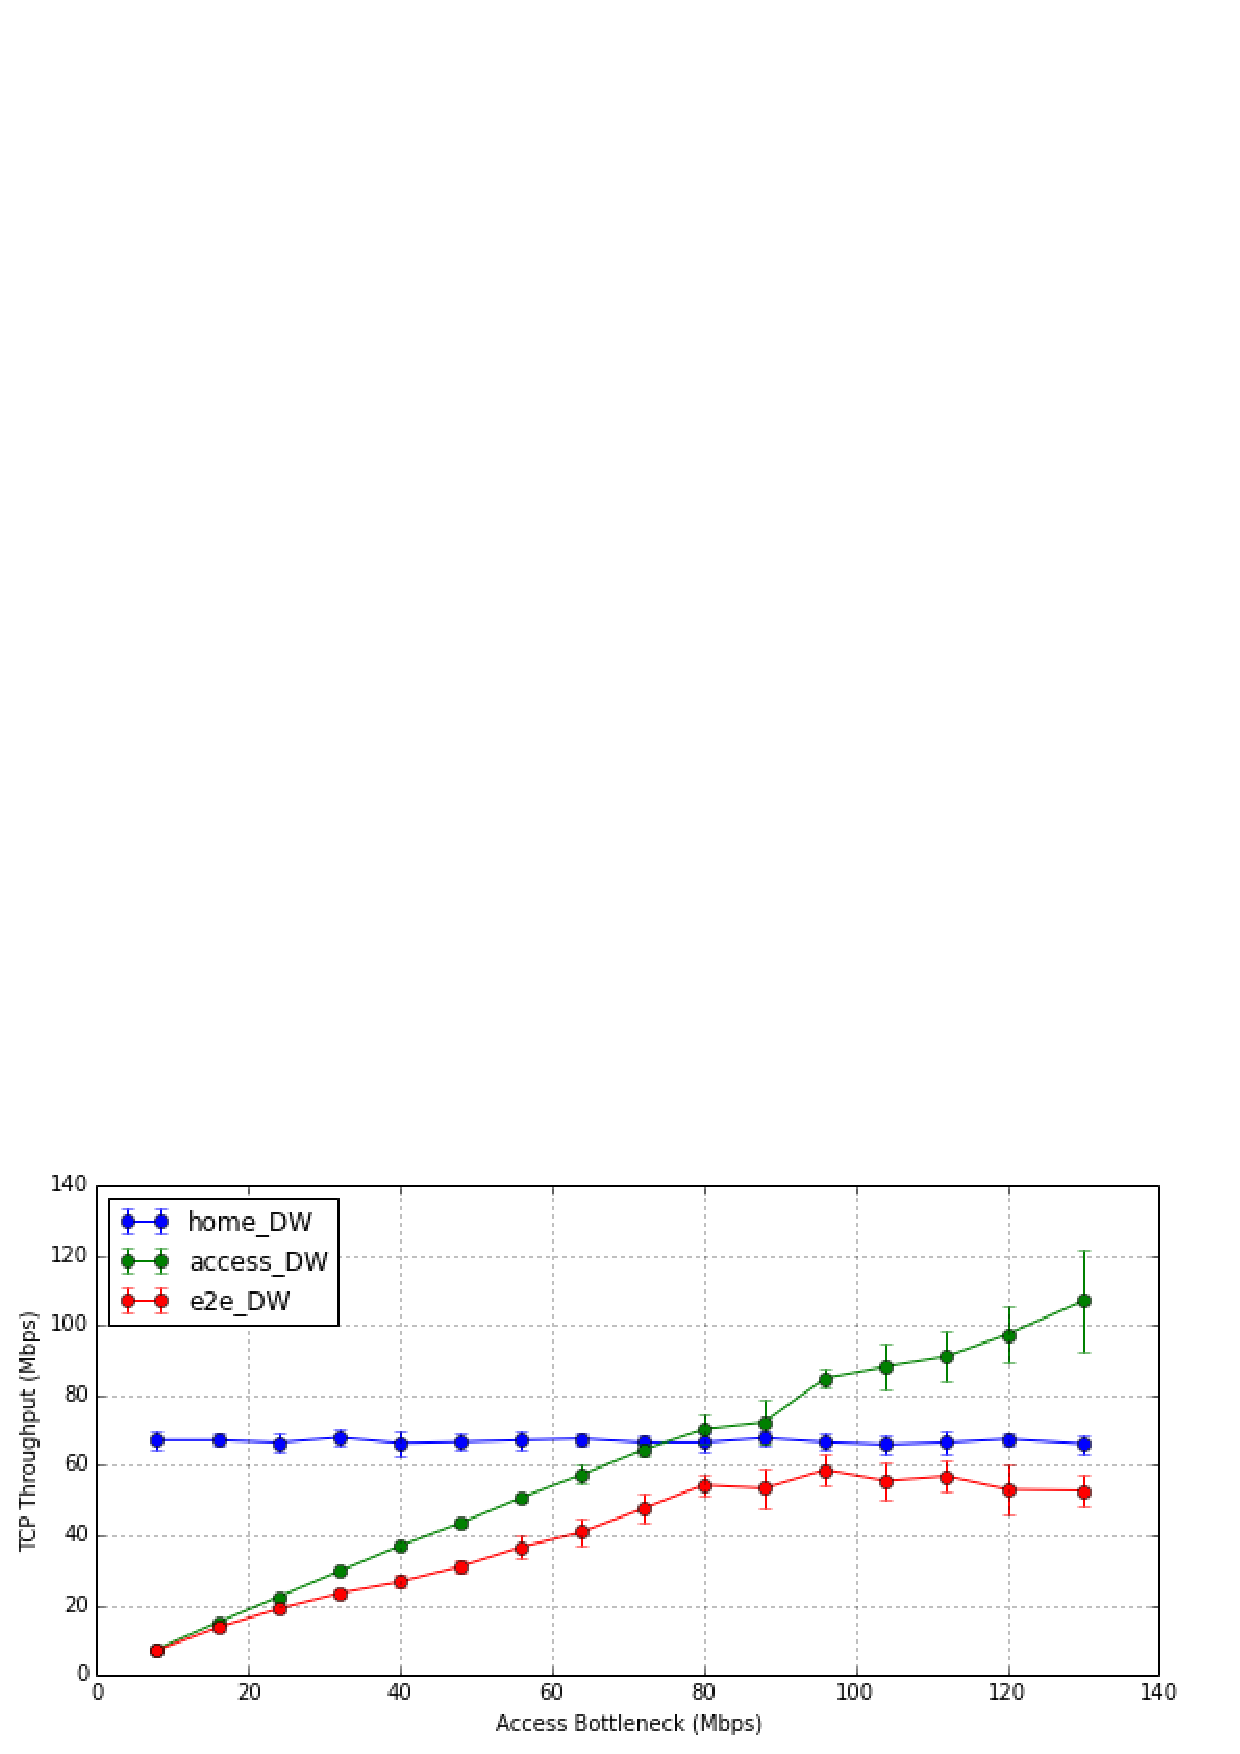
\includegraphics[width=\linewidth]{figures/tcp_throughput_vs_bottleneck.png}
  \caption{Bandwidth measured over each link for a wireless client with a good channel while varying the access link bottleneck}
  \label{fig:throughput_vs_bottleneck}
\end{figure}


%\begin{figure}[!ht]
%\begin{minipage}{.5\textwidth}
%  \centering
%  \includegraphics[width=.4\linewidth]{figures/boxplot_throughput.png}
%  \captionof{figure}{Bandwidth measurements}
%  \label{fig:bandwidth}
%\end{minipage}%
%\begin{minipage}{.5\textwidth}
%  \centering
%  \includegraphics[width=.4\linewidth]{figures/boxplot_latency.png}
%  \captionof{figure}{Latency measurements (confirmed using tcptrace)}
%  \label{fig:latency}
%\end{minipage}
%\end{figure}

%\begin{figure}[!ht]
%  \centering
%  \includegraphics[width=\linewidth]{figures/boxplot_throughput.png}
%  \caption{Bandwidth measurements}
%  \label{fig:bandwidth}
%\end{figure}